\chapter{Concepts and Architecture}
As described in the chapter Related Work, SSB is an ID-centric single feed driven environment, where onboarding is challenging. 
This prerequisite changes from the beginning. The basic idea of the Feed Bundle Protocol is to split up this ID-centric environment into replicated feed-pairs, where two participants hold at least one of such a pair.  This pair contains the whole dialog between two identities which have a contract with each other. Similar to the tin can phone from your childhood, where you had two cans connected for every friend you want to communicate with. By introducing intermediary service providers, the onboarding happens at contract signing. Clients have a possibility to connect to new servers via this ISP and create a new feed-pair for each server, which is replicated over the same ISP. Since this approach means an enormous amount of feed replications between ISP and server, these feeds are bundled again.

\section{Tin Can Analogy}

This system as described may seem difficult to understand, but the description can be simplified. Think of it as a tin can phone from your childhood, but where you have two cans on each side. You need this two-can set up for each friend with whom you want to communicate. You start with a connection to your best friend, the one you trust the most. You talk into the “talk can” and that can ’saves’ everything you say to it. From your other can, the “listen can”, you are only able to hear things from your friend, but this can also saves everything your friend says. By labeling the cans with our names in the format "talker-listener", we distinguish them. The You-Friend can is therefore you "talk can" and your friends "listen can", the Friend-You can the other way around. This is one replicated feed-pair, having both cans on both sides.
\\
Having this, the dialog needs a way or language to express expectations or requests from one side to communicate with each other, where you can declare what you want from your friend, which leads us to the simplified RPC protocol. After a while, it gets boring only talking to this one friend. Luckily, your friend is the coolest kid in school and knows everyone and even tells you about everyone he knows. Then you ask your friend if he could introduce you to his other friends, since you are tired of only talking to your friend. This introduction process is real, human social behavior, not face to face, but via tin can phone.
\\
After your friend has introduced you to one of his other friends and this other friend decides to be friends with you, you and your new friend start to build a new tin can phone, with the “talk can” and “listen can” tins. Due to the fact that you are too far away from each other, you cannot just have a cord from one to the other, so your best friend allows you to route the cord through his house. This corresponds to the replication of the feeds over an intermediary connectivity provider.

Having this, the dialog needs a way or language to express expectations or requests from either side to communicate with each other, where you can declare what you want from your friend. Leading to the simplified RPC protocol.\\ 
There is another problem, however: you are not the only one. After a while, your best friend has so many connections running through his house from all his friends who want to talk to their other friends, that here is an enormous number of strings going to that other friend. Your friend decides to combine all these strings into one and send all messages through this one, single bundled connection, which contains all the information about which tin can it needs to come out of at the end. He multiplexes. Given that little story, we can derive concepts and architecture for the tin can phones of the future.

\begin{figure}
    \centering
    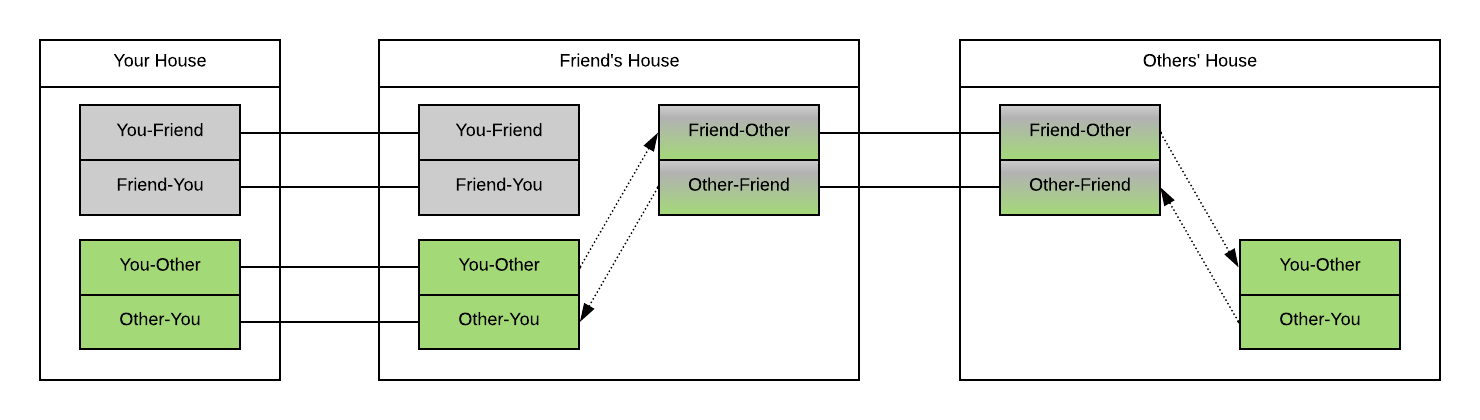
\includegraphics[width=0.9\textwidth]{tincan}
    \caption{Tin can analogy illustrated.}
    \label{fig:tincan}
\end{figure}

\section{Contracts}
Now we can see the foundation of the friendship. The friendship between you and your best friend and the friendship between your best friend and his other friend. By the same token, it is the business contracts between the nodes that provide the foundation for the entire connectivity, protocol and bundling. These contracts are the most important building blocks of the whole thesis since they define the behaviour of the replicated feed-pairs, onboarding mechanics and bundling.

\subsection{Contract Values}
To build the tin can phone, three basic identifiers are needed. First of all, you have to trust each other. This corresponds to the concept of a legal contract between the two parties. Next you need to know the names to label the phones, so you know who you are talking to. These are the public keys. Since everybody in your house can use the tin phone, you also need some sort of code so that your friend knows that it is you who is sending the message and not your mother. These are the private keys. Having that, you need your two tin cans, the feed-pair and two wires, the replication process.
\\
If you do not know your friend’s address, you do not know where to put that wire, so you need some sort of address as well. The address, as the name is well chosen, refers to the IP-address, since this is the most commonly known address of a computer. Last but not least, to distinguish all the cans, you label them corresponding to the "talker-listener" format. Therefore, a contract consists of a public key, a private key, a feed-ID and the peers public key, feed-ID and location. Since a contract has been established, we need to know what happens in the tin cans and the wire. This leads to the replicated feeds. 

\textit{Eventually Picture of identities with contract}

\section{Replicated Feeds}
The following statements can be extracted from the Scuttlebutt Protocol Guide: ”A feed is a signed append-only sequence of messages. Each identity has exactly one feed."\footnote{\url{https://scuttlebot.io/more/protocols/secure-scuttlebutt.html}} and "Messages from feeds 3 hops out are replicated to help keep them available for others."\footnote{\url{https://scuttlebot.io/more/protocols/secure-scuttlebutt.html}} - So what do these properties mean?\\

What can be derived from this information? Signing ensures that you can trust that this message was created by one specific identity or more specifically, the encryption of plain text with the sender’s private key to a cipher text. The crypto text can be deciphered with the sender’s public key.\footnote{quelle} Therefore, this guarantees integrity. Append-only means this sequence can not be forged. So there is no possible way to modify or delete any entries that were appended at any time.\footnote{Feeds - \url{https://ssbc.github.io/scuttlebutt-protocol-guide/}} This append-only property is realized with a mechanism which references the previously generated message.\footnote{Feeds - \url{https://ssbc.github.io/scuttlebutt-protocol-guide/}} The ID-centric architecture described means exactly one identity (key) is mapped to exactly one feed, where every single bit of information an identity creates and "consumes"\footnote{describe better} in the SSB universe is stored in this feed.
\\
There is a lot more going on in the SSB feed and protocol, but an adapted simplified version with three fields\textit{(Figure link and simplify even more)} is more than sufficient for this thesis. 

\begin{figure}
    \centering
    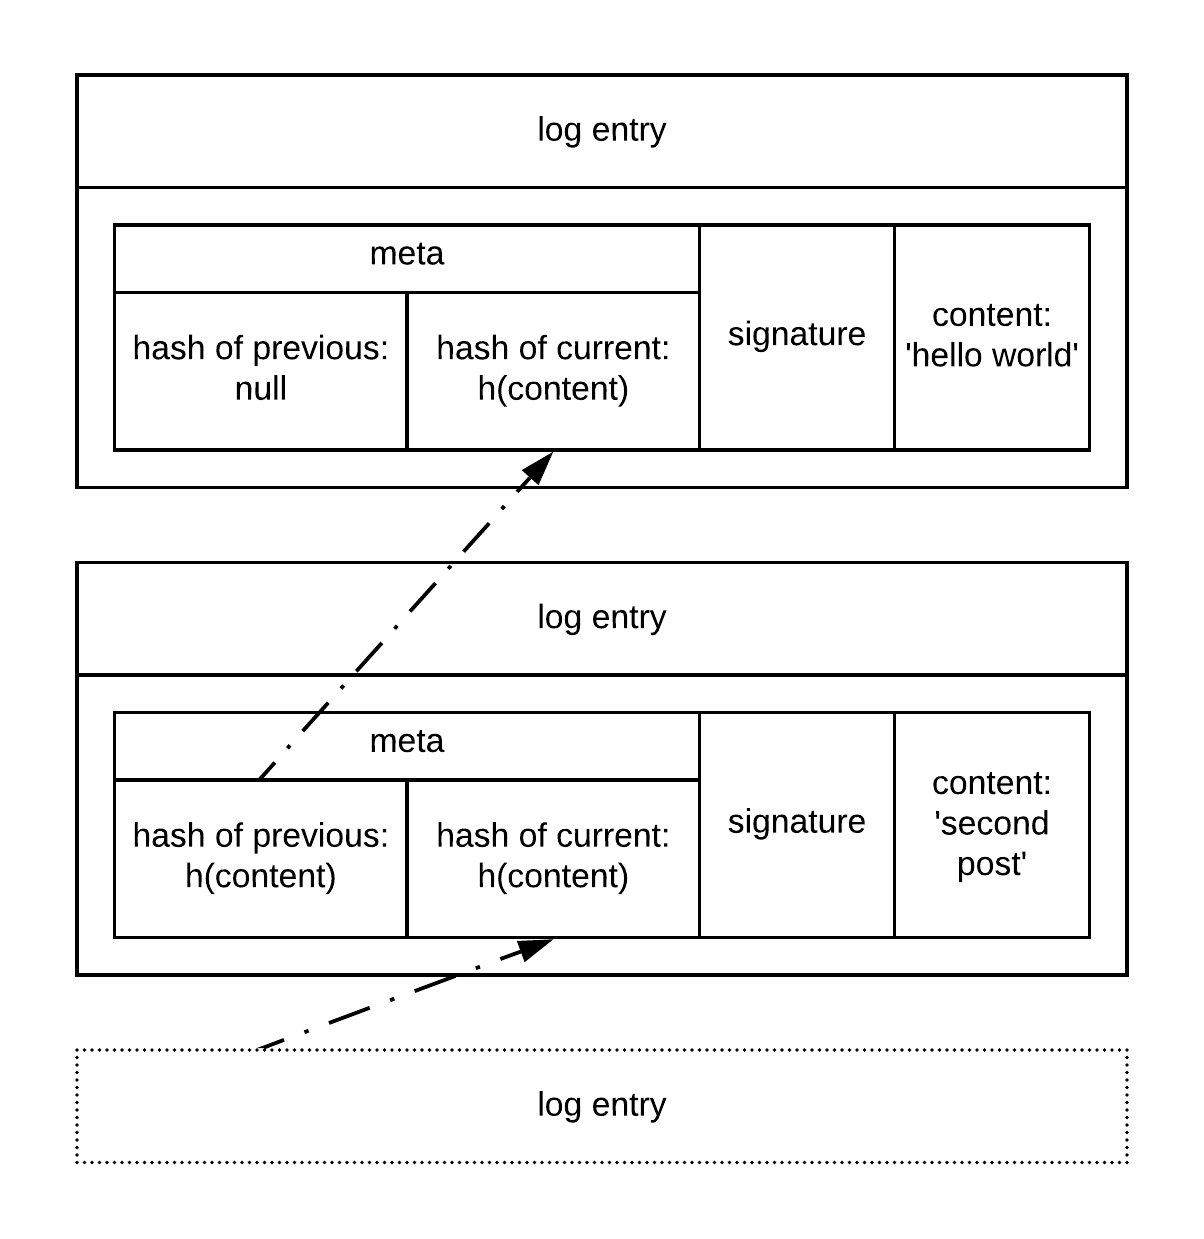
\includegraphics[width=0.5\textwidth]{feed_schema}
    \caption{A schematic simplified feed with the fields meta, signature and content.}
    \label{fig:feed_schema}
\end{figure}



These properties underline the trust by guaranteeing completeness and validity of the information read in a feed. We can, however, see the sticking point in the replication of ID-centric feeds. Since the replication of the SSB protocol always replicates the whole feed with all information to all peers three hops away from a single identity, there is great amount of replication work done. This causes latency and long scuttling time (feed update).\footnote{Quelle} By splitting the feeds into smaller ones and having the effective communication between two parties bundled in the feed pairs mentioned previously, we try to bypass this bottleneck. As a result, we have a diagram like this: For the sake of clarity, only the situation between the client and the ISP is shown. 

\begin{figure}
    \centering
    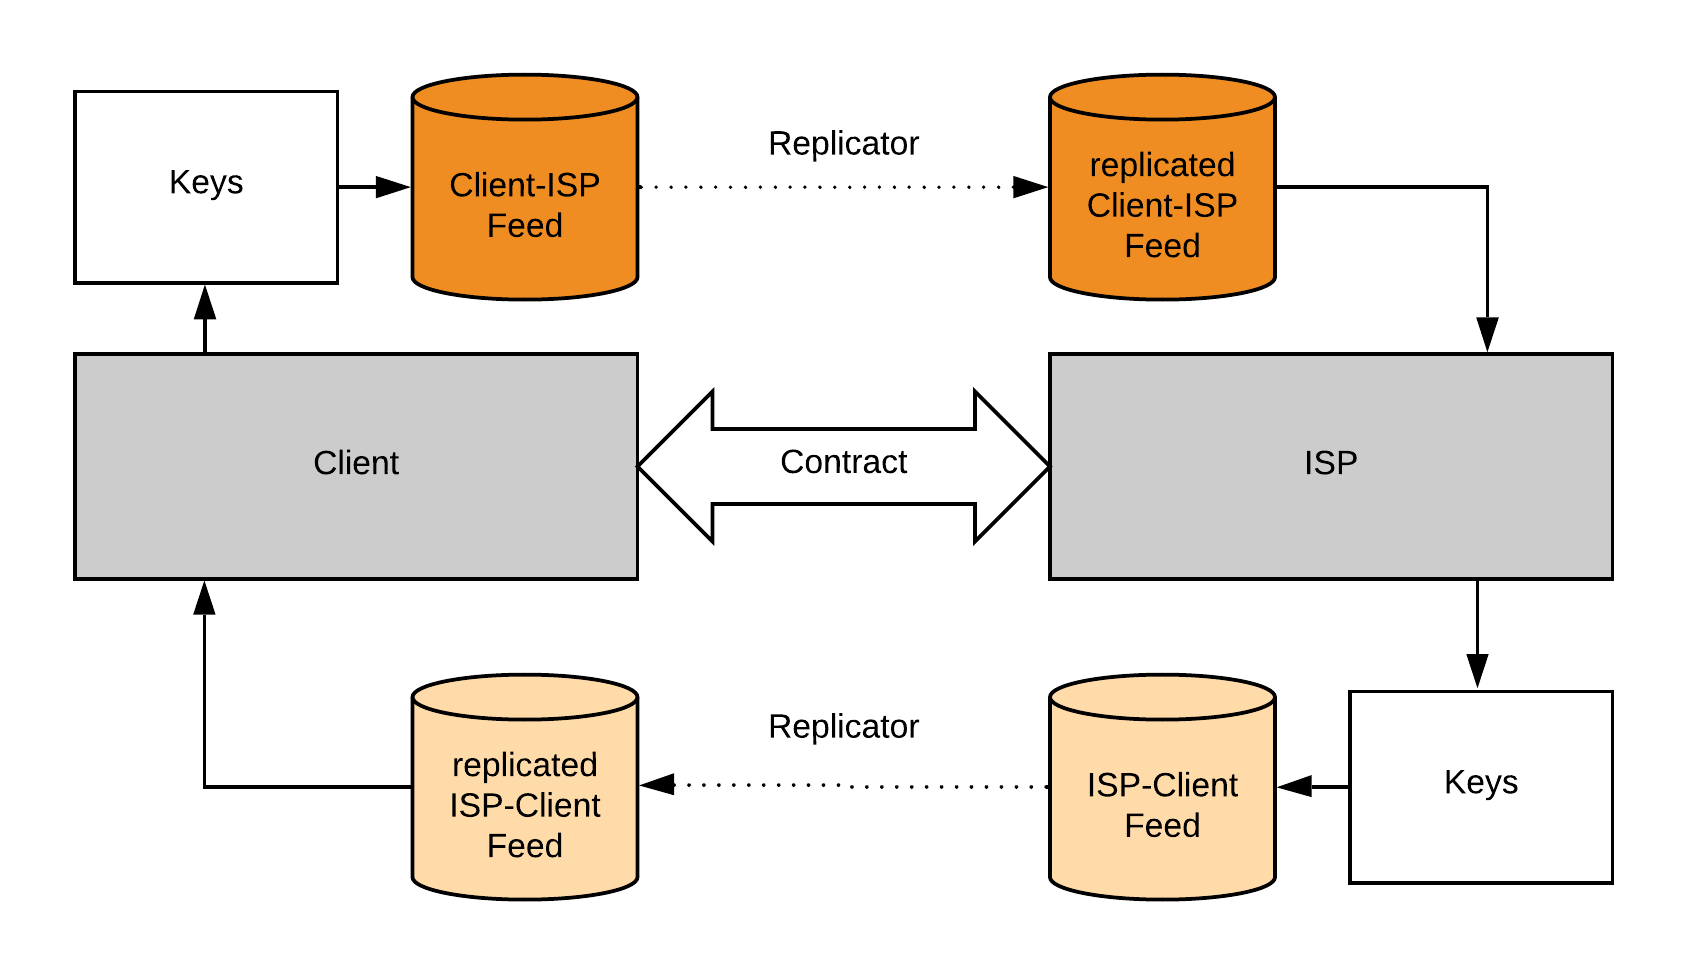
\includegraphics[width=0.9\textwidth]{fbp_v0_1_Schema}
    \caption{Feed-pair between client and ISP.}
    \label{fig:contract_cli_isp}
\end{figure}
The replicator or the replication process has it first appearance. As a concept, there is some sort of replicator instance or procedure that replicates the feeds to the corresponding address or location. Let's take a closer look at the implementation part. \\
Having this setup, the next step is to have a possibility to communicate, so the client can request information from the ISP’s real database.

\pagebreak
\section{Remote Procedure Call}
As explained in the section Related Work, Remote Procedure Calls are a useful paradigm for providing communication across a
network between programs (\citet{birrell1984implementing}). This faces many challenges, but these are not particularly relevant to this stage in the development of the Feed Bundle Protocol. Therefore, the RPC used in this section is a very simplified version.\\
The idea is to have a caller, in our case the client, and a callee, the ISP or server. Having this kind of request–response protocol, an RPC-request is initiated by the caller, which sends a request to a callee in order to execute a specified procedure with given attributes. However, "sending" is not the appropriate terminology for an environment with the replicated feeds. The RPC-request is written in the Caller-Callee feed, which is replicated to the callee. When the replication is complete, the callee is notfied of the feed change and can read the request. After processing the request, the result is written in the Callee-Caller feed and the caller can use the result as needed. In our case, these specified procedures are called services. By having only one such service e.g. the echo-service, which simply echoes the attributes back to the caller, it is ensured the RPC-protocol works as defined. The introducing and detrucing mechanics, described in the next section, can also be summarized in such services, where the caller makes, for example, an RPC-request to the introduce-service with the necessary parameters. 

%\section{v0.2}
%The next step was to include servers with services. Also here the Prerequisite and contract situation changed.
\section{Introducing and Detrucing}
\subsection{Introducing}
Recapping the tin can phone story: The idea of introducing is to get in touch with a new friend, to whom your best friend introduces you. You and your new friend create a new tin can phone. Since the cord is only long enough to reach your best friend, he connects you to your newly acquired friend. Therefore, the general idea of introducing in the context of the feed-bundling protocol, is onboarding to a new server over your ISP. This approach differs from the common publish and subscribe (pub-sub) architecture. Where the server has no choice to decline a client in the pub-sub model, this is the foundation of the introduce-detruce model, by simulating real, human behaviour. A more detailed description: A client writes an RPC-request for the introduce service of his ISP in the Client-ISP feed. This request needs an attribute which specifies the server which the client wants to be introduced to. The ISP invokes the introduce service with this given parameter, which now makes an RPC-request with information about the client and the fact that it wants to introduce itself to the server. By writing in the ISP-Server feed, the server detects the change and has the choice to either accept or decline the introduce inquiry. If the Server accepts the introduction, it will directly create the Server-Client feed which is replicated to the ISP. Afterwards, it sends a confirmation or acceptance back to the ISP to fulfill the request. 
\\
The server can also decline the introducing attempt, which results in a rejection, followed by no contract or some sort of empty contract. Either way, the ISP gets the result and fulfills the initial RPC request. The client now gets their result. Depending on the state of acceptance or rejection, the Client-Server feed, replicated to the ISP in accordance with the contract,is successfully established. If the client wants to use a service from server, it only writes the request in the corresponding feed and the procedure is the same as described in the RPC Section, whereby the feed is just simply forwarded over the ISP. 
An important distinction: only the client can introduce itself. The server has no knowledge of clients and also no way to acquire knowledge of clients, so only the client can ask the server for a contract.

\subsection{Detrucing}
Detrucing as a newly invented word in this thesis, since normally after you introduce yourself to a person, there is no way to make this “un-happen”. It acts the same as an unfollow in a pub-sub domain or as terminating the contract. But contrary to the introduce procedure, both parties of the contract can detruce.
Either the client or the server can send an RPC-request to the ISP service to detruce, which is propagated to the opposite end descibed above in the Introducing section and results in the termination of the whole contract. The result of this action is deleting keys and feeds. There is no way to decline a detruce service request. An important note: after detrucing from either side, the client can yet again introduce itself to the server and the server has the possibility to accept or decline the introduction again.
A new diagram of the network can be derived using these descriptions.
\begin{figure}
    \centering
    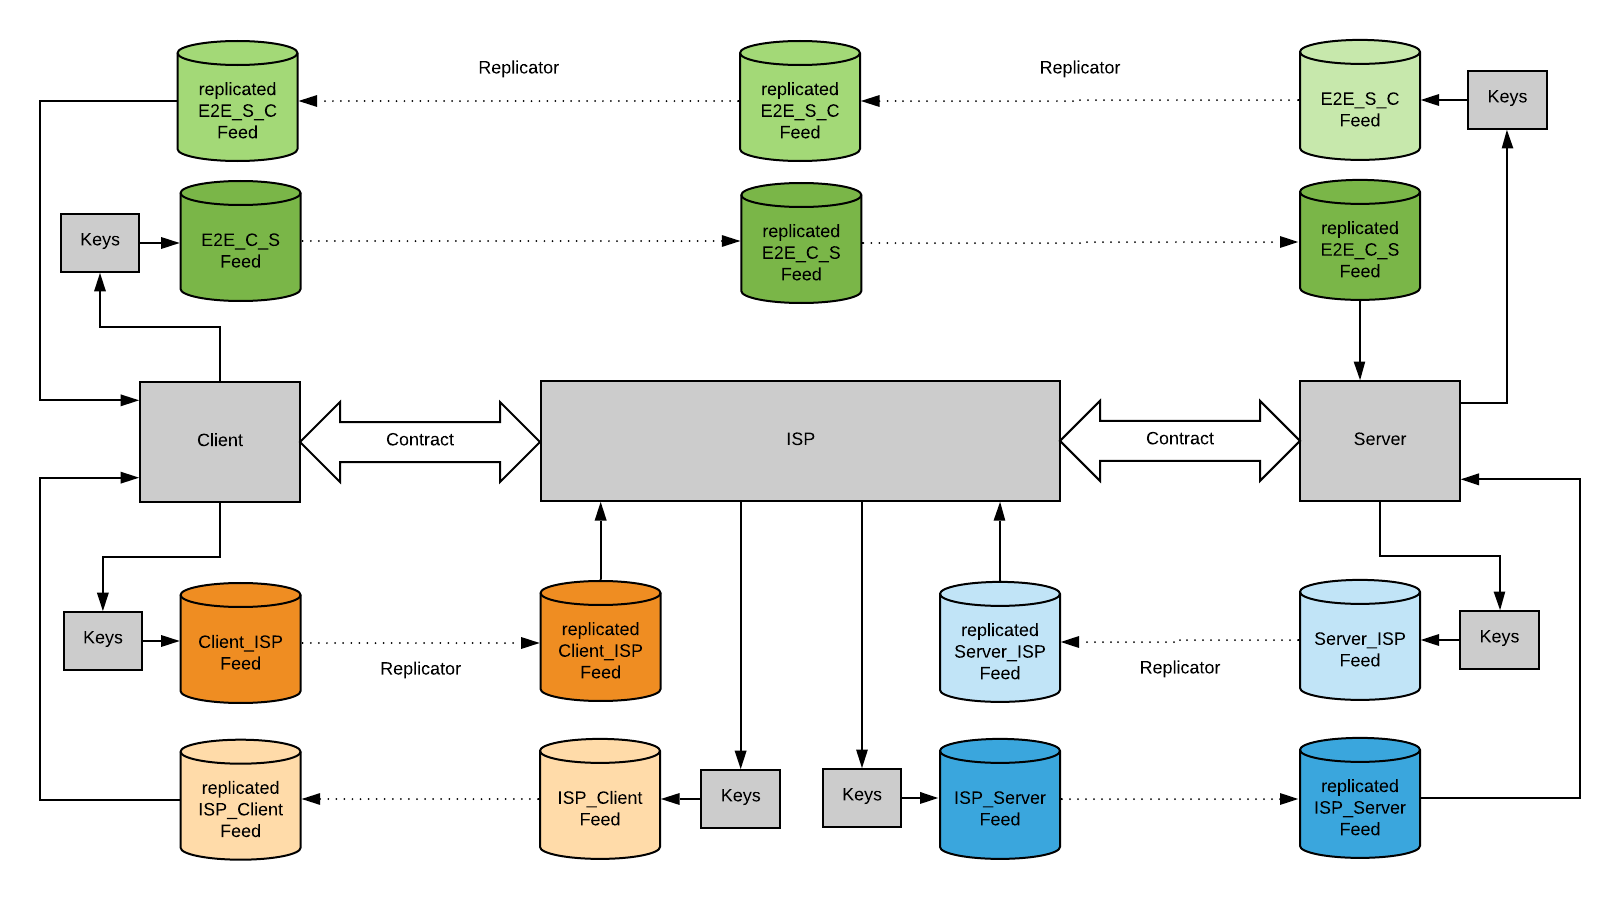
\includegraphics[width=0.9\textwidth]{intro_detru}
    \caption{State after accepted introduce-request from Client to Server. Clearly seen the green End-to-End feed-pair is replicated over the mediating ISP.}
    \label{fig:contract_cli_isp}
\end{figure}

\pagebreak

%\section{0.4}
%added indirect communication from client to server over ISP\\
\section{Bundling}
Taking a look at the real-world problem again, the ISP will have a random number of clients, many of whom want to communicate with the same server. Instead of repeating each End-to-End feed-pair over the ISP to the server, the new requests will be sent through a single feed pair between the ISP and the server. This should reduce the amount of replication work enormously.

\subsection{Adapted Introducing and Detrucing}
The introducing and detrucing idea remains the same, whereby the replication process is
different. After a server accepts a client, the server generates the entire feed pair: Client-Server and Server-Client feed. But instead of replicating to the ISP, nothing happens. To close the introduce request, the server sends the contract to the ISP and the ISP generates the feed there, which holds data from the server to the client: the Server-Client feed. It is the same feed as in the server, but it is not replicated over the general replication instance from server to ISP, it is replicated from the ISP to the client. Finally, the client receives the result and generates the feed, which contains the data from the client to the server: the Client- Server feed. This feed is also replicated the normal way to the ISP. So, the feed-pair for client-server communication is normally replicated between client and ISP, whereas between ISP and server a new way of replication is given.

\begin{figure}
    \centering
    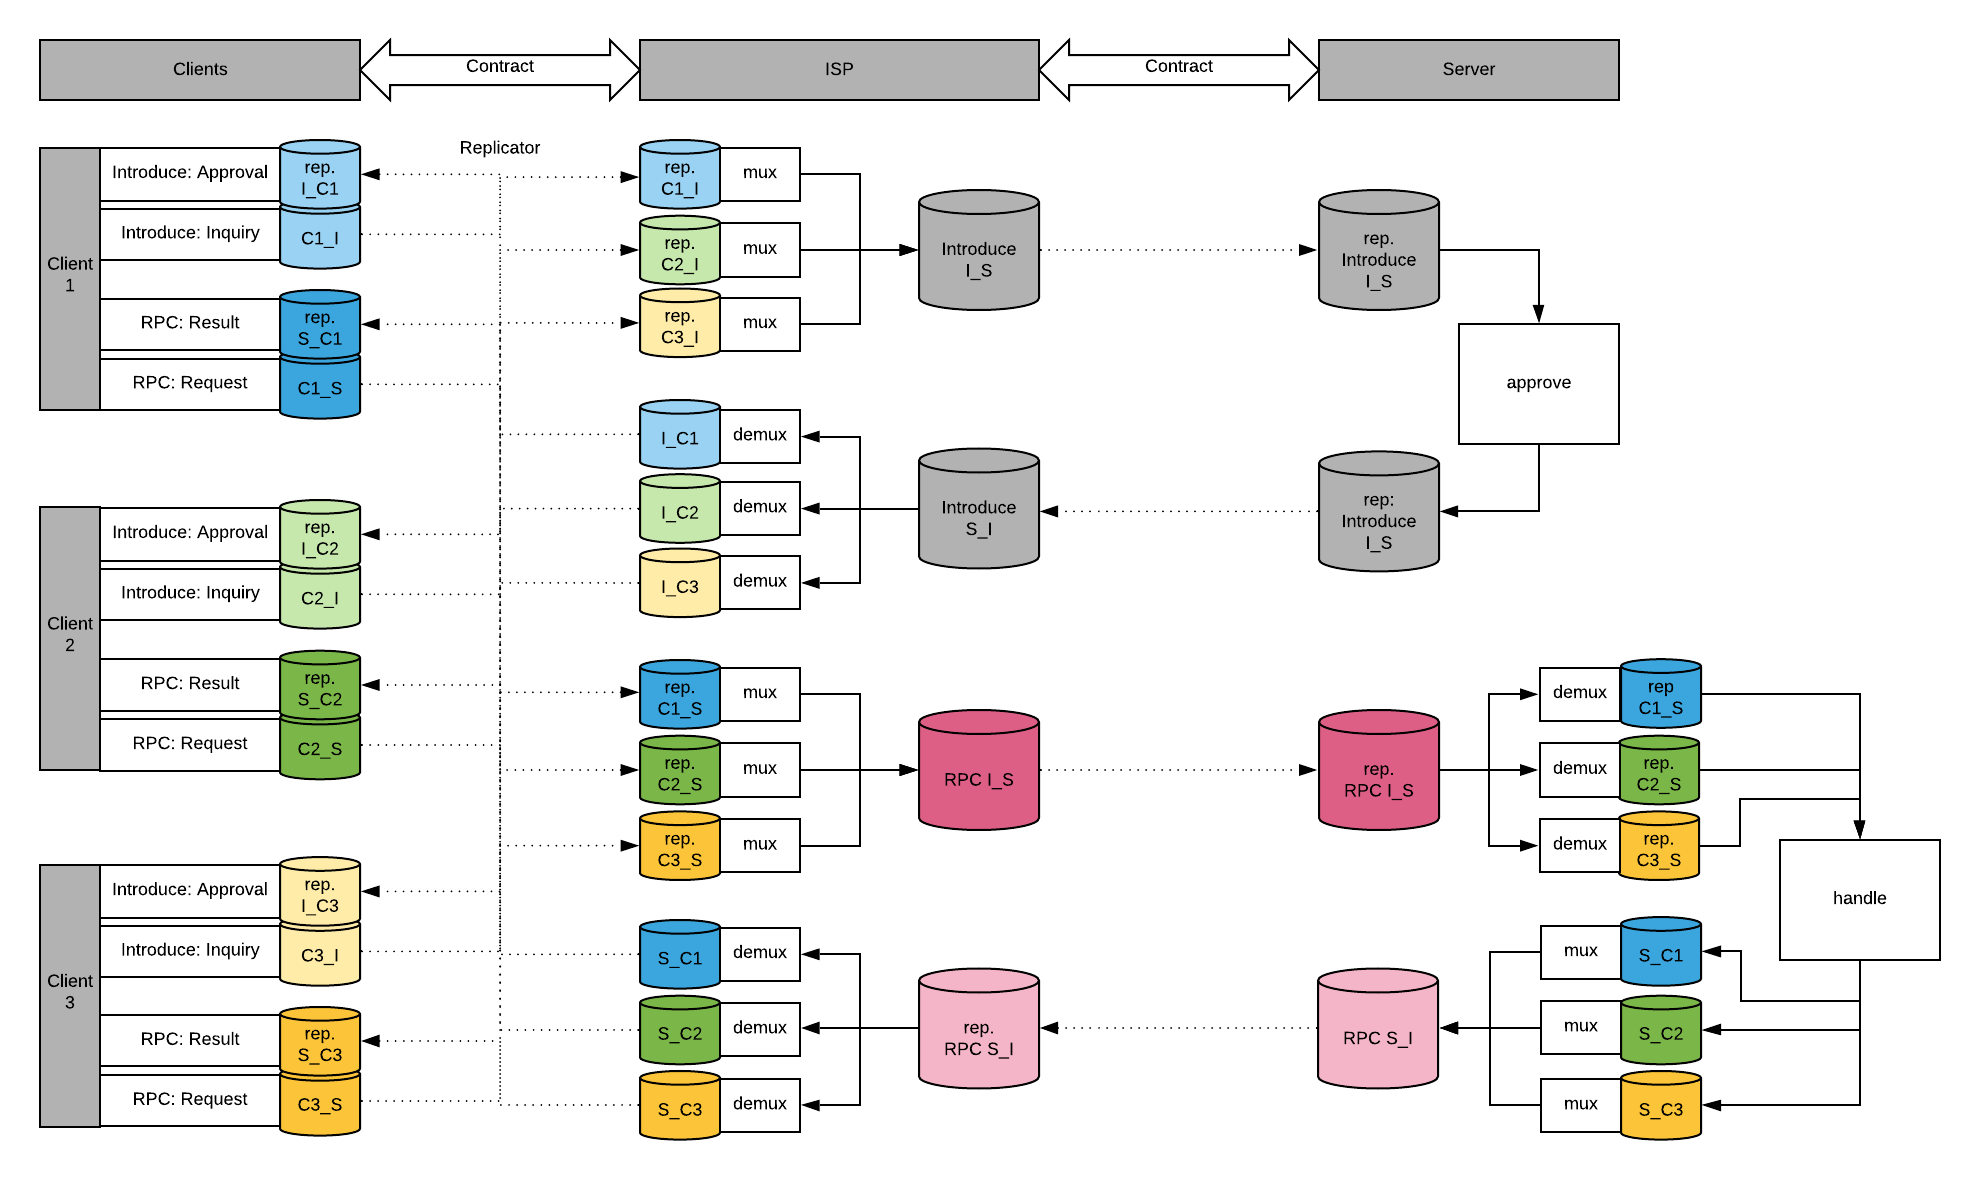
\includegraphics[width=0.9\textwidth]{mux_schema}
    \caption{multiplexing}
    \label{fig:mux}
\end{figure}

\subsection{Multiplexing and Demultiplexing}
As far as the communication between a client and a server is concerned, requests from the client are transferred to the ISP the same way as before. Instead of just forwarding the updated feed, by replicating to the server, the ISP detects new log entries and multiplexes these into a new log entry.
More specifically, the ISP generates a log entry signed by itself, containing the whole log entry signed by the client. This log entry is written to the ISP-Server feed and replicated. The server detects the change on the ISP-Server feed and takes this log entry. The multiplexed log entry, which belongs into a client-server feed, is extracted and appended to the Client-Server feed. This step is called demultiplexing. At this point, the situation is the same as before. A change in the Client-Server feed is given and the request is executed. The result is written to the Server-Client feed and not replicated again over the ISP directly to the client. From there, the whole story is repeated. The log entry is multiplexed once again in the Server-ISP feed and when it arrives at the ISP, it is demultiplexed and appended to the Server-Client feed. From there, it is replicated to the client and the client receives its result for the request.
\begin{figure}
    \centering
    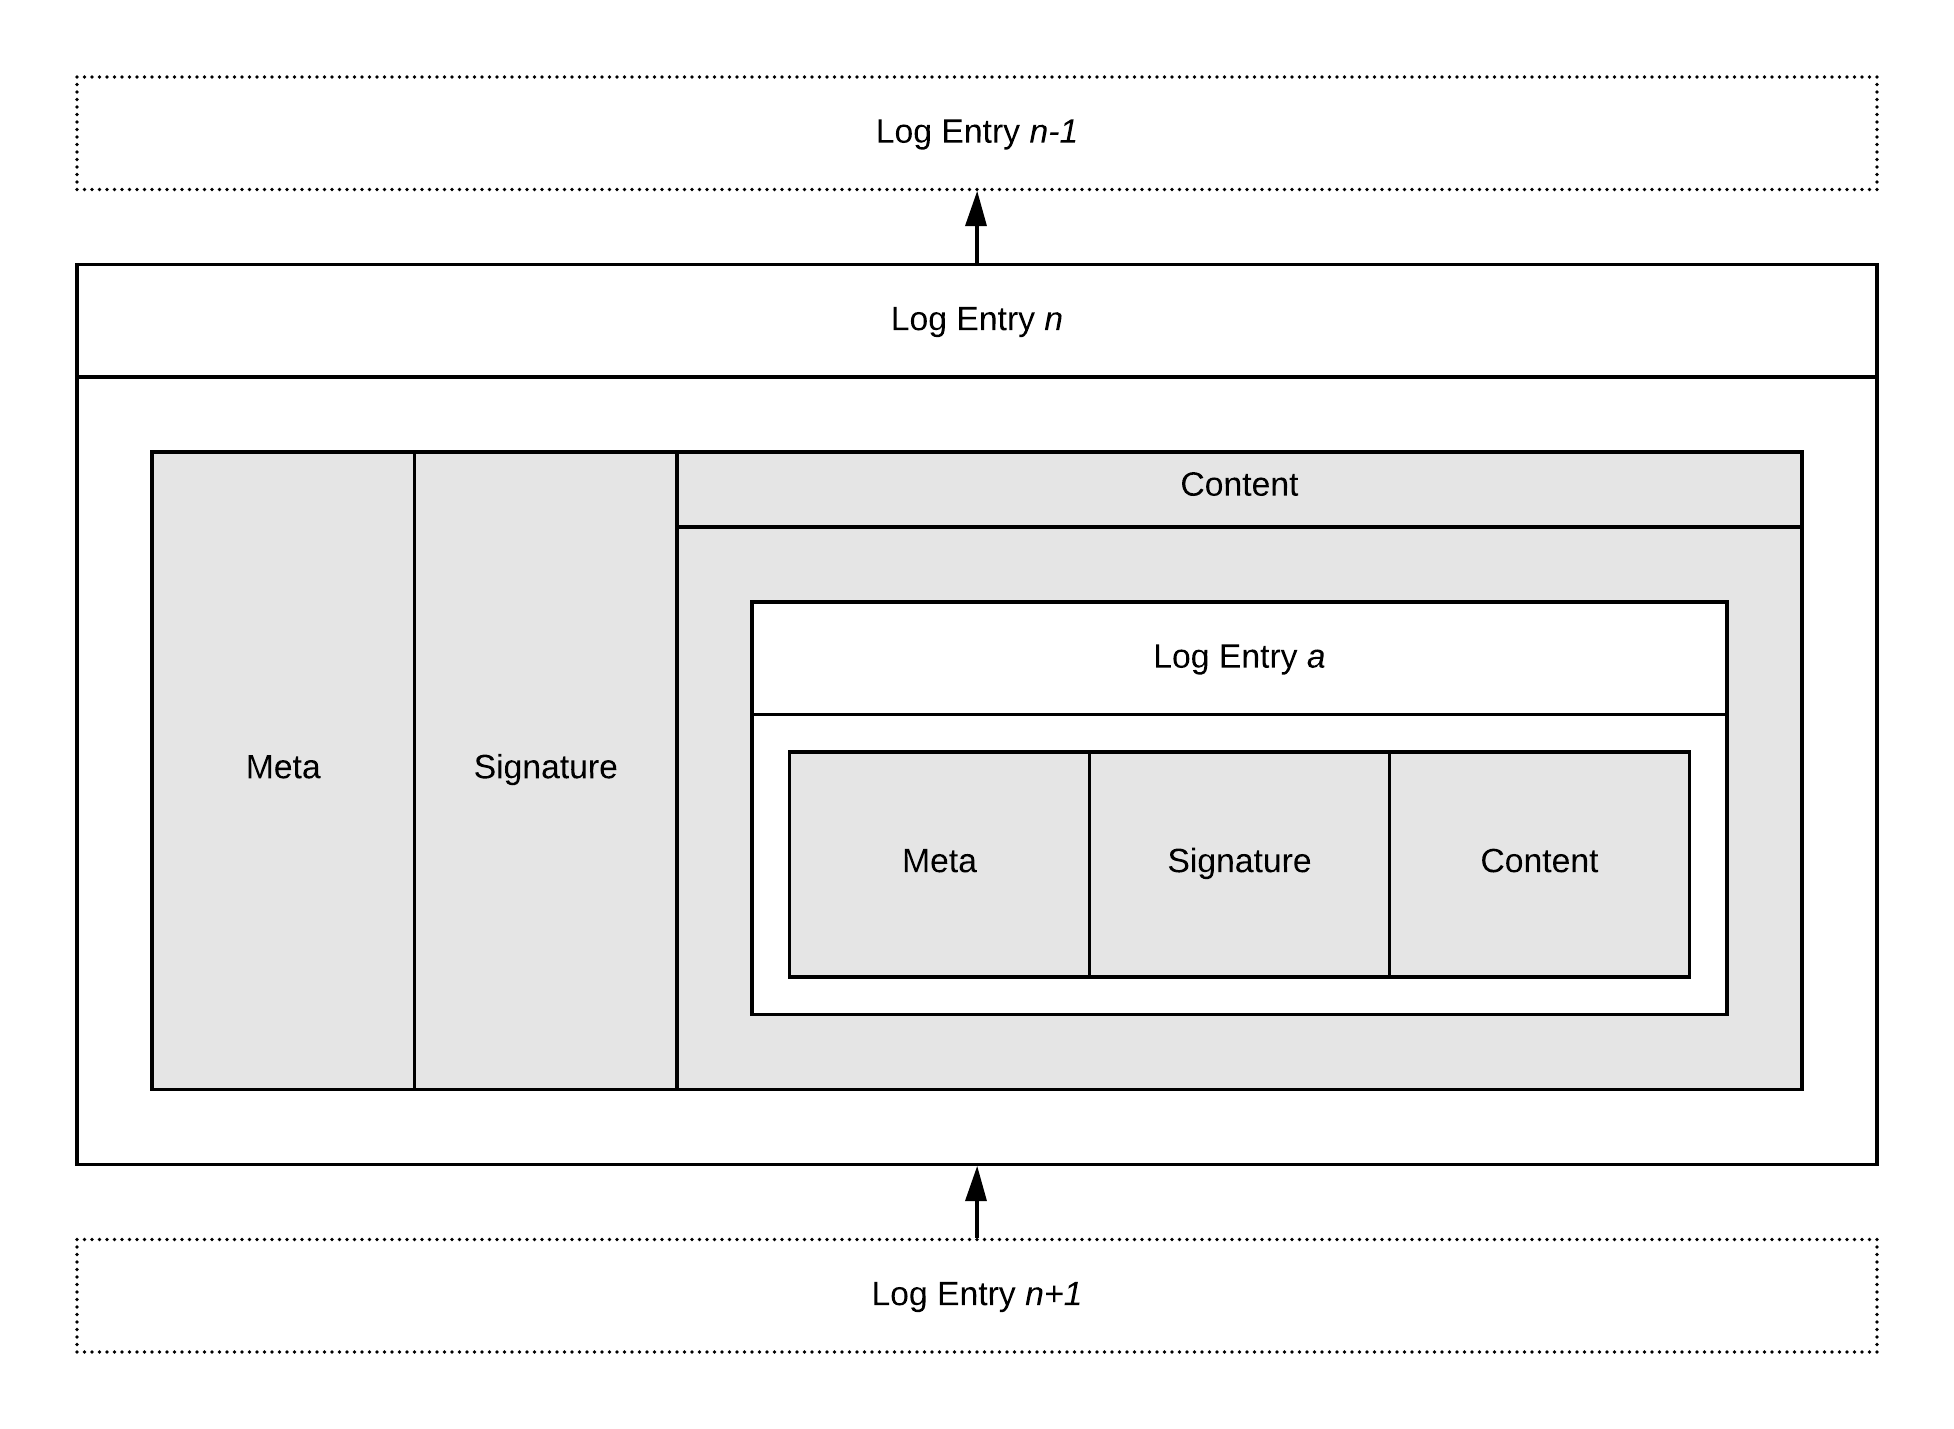
\includegraphics[width=0.9\textwidth]{loginlog}
    \caption{A log entry inside another log entry.}
    \label{fig:loginlog}
\end{figure}


\section{Outlook}
Having all these concepts and architecture, we see the whole process is simplified on a single central ISP. In the real world, this is not the case, but as proof of concept it is more than sufficient. In the next steps, the system must be expanded by splitting this same internet service provider into a network of internet connectivity providers, which act as effective connectivity stations. An additional architecture must be developed where clients and servers can connect to these connectivity nodes. Adding more ISPs necessarily means that more internet service provider companies will be needed. The dynamic of contracts between ISPs will be explored, but more in the Future Work section.